
%(BEGIN_QUESTION)
% Copyright 2015, Tony R. Kuphaldt, released under the Creative Commons Attribution License (v 1.0)
% This means you may do almost anything with this work of mine, so long as you give me proper credit

Calculate the output voltage of this opamp circuit assuming a constant input voltage of +1.5 volts applied for 0.5 seconds.  Assume the capacitor begins in a state of zero charge ($V_0$ = 0 volts):

$$\includegraphics[width=15.5cm]{i01026x01.eps}$$

Also, calculate the ``time constant'' of this integrator circuit (i.e. the factor relating output voltage rate-of-change to input voltage).

\underbar{file i01026}
%(END_QUESTION)





%(BEGIN_ANSWER)

$$V_{out} = -{1 \over RC} \int_{t_0}^{t_f} V_{in} \> dt + V_0$$

$$V_{out} = -\left({1 \over (270 \times 10^3 \> \Omega)(0.33 \times 10^{-6} \hbox{ F})}\right) \left( \int_{0}^{0.5} 1.5 \> dt \right) + 0 \hbox{ V}$$

$$V_{out} = - \left( {1 \over 0.0891 \hbox{ s}} \right) (0.75 \hbox{ V} \cdot \hbox{s}) + 0 \hbox{ V}$$

$$V_{out} = - 8.418 \hbox{ V}$$

\vskip 10pt

Calculating the time constant for this integrator circuit:

\vskip 10pt

$\tau_i = RC = (270 \times 10^3 \> \Omega)(0.33 \times 10^{-6} \hbox{ F}) = 0.0891 \hbox{ seconds}$

%(END_ANSWER)





%(BEGIN_NOTES)


%INDEX% Electronics review: integrator circuit

%(END_NOTES)


